%%%%%%%%%%%%%%%%%%%%%%%%%%%%%%%%%%%%%%%%%%%%%%%%%%%%%%%%%%%%%%%%%%%%%%%%%%%%%%%%
\chapter{Разработка прототипа}
%%%%%%%%%%%%%%%%%%%%%%%%%%%%%%%%%%%%%%%%%%%%%%%%%%%%%%%%%%%%%%%%%%%%%%%%%%%%%%%%
В данном разделе описываются значимые детали реализации прототипа метода редукции программ на языке Kotlin. Основное применение прототипа --- локализация ошибок компилятора языка Kotlin. Кроме данного раздела, еще одним источником информации является исходный код прототипа, частично представленный в приложении~2.

%%%%%%%%%%%%%%%%%%%%%%%%%%%%%%%%%%%%%%%%%%%%%%%%%%%%%%%%%%%%%%%%%%%%%%%%%%%%%%%%
\section{Архитектура прототипа}
%%%%%%%%%%%%%%%%%%%%%%%%%%%%%%%%%%%%%%%%%%%%%%%%%%%%%%%%%%%%%%%%%%%%%%%%%%%%%%%%
Разработанный на языке Kotlin прототип основывается на предложенной технологии программной редукции. Общая структура пакетов представлена на рисунке~\ref{packages}. Как видно из диаграммы, прототип состоит из следующих основных частей:
%
\begin{itemize}
	\item \texttt{manager} --- отвечает за запуск трансформаций и обработку результатов;
	\item \texttt{parser} --- отвечает за построение синтаксического дерева;
	\item \texttt{passes} --- содержит реализацию всех трансформаций;
	\item \texttt{util} --- содержит вспомогательные компоненты.
\end{itemize}
%
Далее реализация прототипа будет рассмотрена более детально.

\begin{figure}
\center{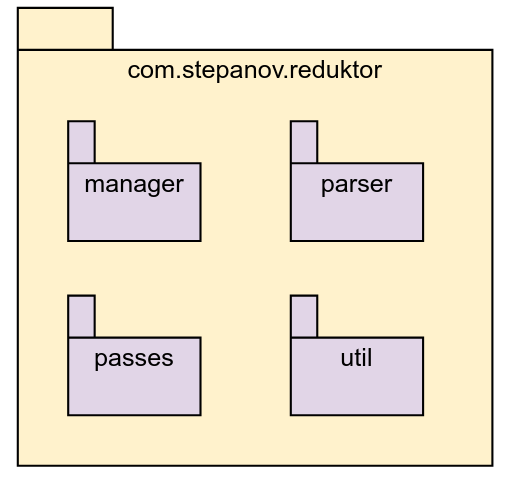
\includegraphics[width=0.5\linewidth]{fig/packages}}
\caption{\label{packages}Общая структура пакетов прототипа}
\end{figure}

%%%%%%%%%%%%%%%%%%%%%%%%%%%%%%%%%%%%%%%%%%%%%%%%%%%%%%%%%%%%%%%%%%%%%%%%%%%%%%%%
\section{Реализация инструмента для построения синтаксического дерева}
%%%%%%%%%%%%%%%%%%%%%%%%%%%%%%%%%%%%%%%%%%%%%%%%%%%%%%%%%%%%%%%%%%%%%%%%%%%%%%%%
В пакете \texttt{parser} содержится код, предназначенный для построения СД из исходного кода на языке программирования Kotlin. Построение производится путем использования инструментария компилятора Kotlin. Для каждого файла с исходным кодом строится свое СД. Можно отметить, что для обхода СД и его редактирования также используется функциональность компилятора Kotlin.

Как было написано ранее, язык программирования Kotlin полностью совместим с языком Java. В качестве дополнительной функциональности было реализовано получение СД для кода на языке программирования Java, так как большое количество программ являются мультиплатформенными, то есть имеющими код как на языке Kotlin, так и на языке Java. Для редукции таких проектов будет необходимо обрабатывать и код на языке Java. В разрабатываемом прототипе к Java-файлам могут применяться трансформации над текстовым представлением и иерархический дельта дебаггинг.

%%%%%%%%%%%%%%%%%%%%%%%%%%%%%%%%%%%%%%%%%%%%%%%%%%%%%%%%%%%%%%%%%%%%%%%%%%%%%%%%
\section{Реализация редуцирующих трансформаций}
%%%%%%%%%%%%%%%%%%%%%%%%%%%%%%%%%%%%%%%%%%%%%%%%%%%%%%%%%%%%%%%%%%%%%%%%%%%%%%%%
В пакете \texttt{passes} содержатся все редуцирующие трансформации. Каждая трансформация принимает на вход какое-либо представление кода и всю необходимую информацию и обрабатывает его. На выходе трансформация производит программу, которая приводит к той же ошибке, что и поданная на вход, но имеющую меньший размер. Все реализованные алгоритмы соответствуют описанным в предыдущем разделе. Ниже приведены особенности реализации некоторых из них.

Класс \texttt{ParallelHierarchialDeltaDebugging} реализует параллельный иерархический дельта дебаггинг СД путем запуска в отдельных потоках обработки различных уровней дерева. Эксперименты показали, что данная доработка не ускоряет работу метода из-за того, что при удалении более высокоуровневой вершины дерева происходит исключение из обработки большого количества низкоуровневых. Почти всегда количество обрабатываемых дополнительно низкоуровневых элементов настолько велико, что оно перекрывает преимущества параллельной обработки. Возможный путь решения данной проблемы --- при удалении какого-либо элемента сообщать об этом всем элементам нижнего уровня и исключать их из рассмотрения; при этом редукцию на этих уровнях нужно будет запускать заново. Из-за этого распараллеливание дельта дебаггинга на уровнях СД можно считать нецелесообразным.

Класс \texttt{PeepholePasses} реализует все алгоритмы редукции текстового представления программы. Шаблоны, описанные в предыдущем разделе, задаются при помощи регулярных выражений\footnote{https://kotlinlang.org/api/latest/jvm/stdlib/kotlin.text/-regex/index.html}. Единственная проблема, возникшая в процессе разработки, --- скобки могут быть несбалансированными. Для этого они должны находиться либо в строковых константах, либо в названии функций. Такие скобки не учитываются.

Класс \texttt{PreliminarySimplification} реализует алгоритм предварительного упрощения файлов. Данный алгоритм может быть эффективно распараллелен, так как каждый файл обрабатывается независимо. Сначала производится обход дерева зависимостей и формирование выборок файлов и последовательности их запуска. Затем каждый файл в сформированных выборках запускается на упрощение в отдельном потоке.

%%%%%%%%%%%%%%%%%%%%%%%%%%%%%%%%%%%%%%%%%%%%%%%%%%%%%%%%%%%%%%%%%%%%%%%%%%%%%%%%
\subsection{Пакет \texttt{com.stepanov.reduktor.passes.slicer}}
%%%%%%%%%%%%%%%%%%%%%%%%%%%%%%%%%%%%%%%%%%%%%%%%%%%%%%%%%%%%%%%%%%%%%%%%%%%%%%%%
Данный пакет содержит в себе классы, реализующие алгоритмы программных срезов, описанные в предыдущем разделе. Пакет содержит класс \texttt{Slicer}, который принимает на вход номер строки с ошибкой и запускает выбранный вид слайсинга. Для получения переменных по номеру строки была написана функция \texttt{getline}, которая извлекает из текстового представления программы содержимое заданной строки и с помощью инструментария компилятора Kotlin строит для него выражение.

Как было описано ранее, внутрипроцедурный слайсер обходит тело функции снизу вверх и удаляет все то, что не относится к критерию среза. Данный проход имеет несколько особенностей в его реализации:
\begin{itemize}
	\item если в критерии среза содержится номер строки, указывающей на вызов функции, то в качестве переменных в критерии среза используются аргументы, переданные в функцию;
	\item если известна только функция, в которой содержится ошибка, то поочередно производится срез относительно каждой строки этой функции. При неудачном воспроизведении ошибки программа откатывается к предыдущему состоянию и производится переход на следующую строку;
	\item для безопасности слайсинга определен четкий набор обрабатываемых видов выражений (унарное, бинарное, вызов функции и т.д.), также обрабатываются операторы перехода.
\end{itemize}

Слайсер на уровне функций работает по алгоритму, описанному в разделе~\ref{slicingalg}, --- он строит дерево использований функций, где корнем является функция с ошибкой, фильтрует рекурсивные вызовы и удаляет все функции, которые не попали в это дерево. Для реализации построения дерева необходимо соотнести вызов функции с ее сигнатурой. Для этого необходимо провести анализ кода. Однако при редукции компиляторных ошибок часто он не может быть проведен, и поэтому у нас не имеется никакой информации о типах аргументов в вызове функции, если только они не указаны явно. Для решения этой проблемы была написана функция \texttt{getSignature}, которая считает количество аргументов, и дальнейший поиск производится по имени функции и количеству ее аргументов. Очевидно, что иногда такой подход будет строить неверные деревья, поэтому после удаления каждой функции производится проверка корректности проведенной трансформации.

%%%%%%%%%%%%%%%%%%%%%%%%%%%%%%%%%%%%%%%%%%%%%%%%%%%%%%%%%%%%%%%%%%%%%%%%%%%%%%%%
\section{Реализация менеджера проходов}
%%%%%%%%%%%%%%%%%%%%%%%%%%%%%%%%%%%%%%%%%%%%%%%%%%%%%%%%%%%%%%%%%%%%%%%%%%%%%%%%
В пакете \texttt{reducer} содержится компонент \texttt{TransformationManager}, реализующий управление всеми трансформациями. Данный компонент осуществляет запуск наборов трансформаций для проектов (\texttt{doProjectTransformations}) и отдельных файлов (\texttt{doTransformations}). Трансформации запускаются в цикле до тех пор, пока файл с ошибкой не перестанет изменяться. Также данный компонент отвечает за пост-обработку результатов --- форматирование и сохранение. Для форматирования результирующего кода был апробирован проект ktlint\footnote{https://github.com/shyiko/ktlint}, но его применение не дало ожидаемых результатов. После этого была попытка интегрировать модуль редактирования стиля кода из среды разработки IDEA\footnote{https://www.jetbrains.com/idea/} и компилятора Kotlin, но ввиду сложности внутренних связей данного модуля интеграция является слишком ресурсозатратной. Поэтому была реализована простая трансформация, удаляющая лишние переводы строк. Создание трансформации для форматирования результирующего кода является одним из направлений дальнейшей работы.

%%%%%%%%%%%%%%%%%%%%%%%%%%%%%%%%%%%%%%%%%%%%%%%%%%%%%%%%%%%%%%%%%%%%%%%%%%%%%%%%
\section{Реализация вспомогательных компонентов}
%%%%%%%%%%%%%%%%%%%%%%%%%%%%%%%%%%%%%%%%%%%%%%%%%%%%%%%%%%%%%%%%%%%%%%%%%%%%%%%%
Пакет \texttt{util} содержит вспомогательные компоненты, решающие следующие задачи:
\begin{itemize}
	\item запуск программы и проверка воспроизведения ошибки --- \texttt{CompilerCrashTestChecker} и \texttt{TestChecker};
	\item хранение аргументов, с которым запускается компилятор --- \texttt{CompilerArgs};
	\item разбор сообщения об ошибке и ее хранение --- \texttt{Error};
	\item распараллеливание задач предварительного упрощения на уровне файлов --- \texttt{ParallelFileProcessingUtil};
	\item удаление файлов исходного кода из архива с зависимостями --- \texttt{RemoveSourcesFromJar};
	\item дополнительные инструменты для редактирования СД --- \texttt{Extensions}.
\end{itemize}
Ниже приведено описание наиболее интересных компонентов.

%%%%%%%%%%%%%%%%%%%%%%%%%%%%%%%%%%%%%%%%%%%%%%%%%%%%%%%%%%%%%%%%%%%%%%%%%%%%%%%%
\subsection{Компоненты \texttt{CompilerCrashTestChecker} и \texttt{TestChecker}}
%%%%%%%%%%%%%%%%%%%%%%%%%%%%%%%%%%%%%%%%%%%%%%%%%%%%%%%%%%%%%%%%%%%%%%%%%%%%%%%%
Компонент \texttt{TestChecker} позволяет задать желаемый критерий редукции с помощью bash-скрипта~\cite{blum2008linux}. Так как основным применением разработанного прототипа является редукция программ, приводящих к ошибкам компилятора, был разработан отдельный компонент для запуска программ и проверки воспроизведения ошибок, называемый \texttt{CompilerCrashTestChecker}. Для запуска программы используется компонент \texttt{K2JVMCompiler} из компилятора языка Kotlin. С помощью компонента \texttt{CompilerArgs} задаются все необходимые аргументы и производится запуск компилятора с использованием библиотеки \texttt{java.util.concurrent}. Результат запуска сохраняется в специальную структуру \texttt{MessageCollector}, содержащую всю необходимую информацию об ошибке. Далее происходит разбор ошибки и сравнение ее с исходной. В том случае, если сообщение об ошибке не подходит ни под один заданный шаблон, сравниваются текстовые представления ошибок алгоритмом, описанным в разделе~\ref{errorscheck}. Для сравнения используется библиотека \texttt{DiffMatchPatch}, после чего считается коэффициент схожести файлов и сравнивается с заданным ранее коэффициентом~(1.5).

В описываемом компоненте содержатся две доработки для многократного повышения скорости работы прототипа. Первая --- сохранение уже проверенных тестов. Для этого используется таблица, содержащая хэш-код проверенных тестовых примеров и результат их проверки. Второй --- проверка синтаксической корректности запускаемого теста; если тест некорректен, он пропускается. Для данной проверки используется инструментарий компилятора Kotlin: если текст программы некорректен, синтаксическое дерево для нее содержит специальный вид узлов, сигнализирующих об этом. 

%%%%%%%%%%%%%%%%%%%%%%%%%%%%%%%%%%%%%%%%%%%%%%%%%%%%%%%%%%%%%%%%%%%%%%%%%%%%%%%%
\subsection{Компонент \texttt{ParallelFileProcessingUtil}}
%%%%%%%%%%%%%%%%%%%%%%%%%%%%%%%%%%%%%%%%%%%%%%%%%%%%%%%%%%%%%%%%%%%%%%%%%%%%%%%%
Данный компонент реализует параллельный запуск задач на выполнение. Для распараллеливания используется пакет \texttt{java.util.concurrent}, содержащий все необходимые для этого инструменты. Количество создаваемых потоков равно количеству процессоров компьютера. Для каждого потока создается копия проекта, после обработки новый файл сохраняется в старый проект. В проекте используются два вида параллельных задач: быстрое упрощение и набор трансформаций, описанных в компоненте \texttt{PreliminarySimplification}. Быстрое упрощение состоит в попытке замены тел всех функций в файле на вызов специальной функции \texttt{TODO()}. Таким образом в случае, если все функции не влияют на воспроизведение ошибки, производится удаление их тел, что значительно уменьшает размер обрабатываемого кода. 

%%%%%%%%%%%%%%%%%%%%%%%%%%%%%%%%%%%%%%%%%%%%%%%%%%%%%%%%%%%%%%%%%%%%%%%%%%%%%%%%
\subsection{Компонент \texttt{RemoveSourcesFromJar}}
%%%%%%%%%%%%%%%%%%%%%%%%%%%%%%%%%%%%%%%%%%%%%%%%%%%%%%%%%%%%%%%%%%%%%%%%%%%%%%%%
При запуске программы для проверки воспроизведения ошибки компоненту~\texttt{K2JVMCompiler} необходимо передать архив со всеми зависимостями целевого проекта. Данный архив практически всегда содержит и скомпилированный исходный код программы. Это приводит к тому, что при удалении какого-либо компонента программы из исходного кода, он все равно <<подхватывается>> из указанного архива. Описанная ситуация приводит к невозможности воспроизведения ошибки результирующим тестовым примером. Данный компонент занимается удалением всех скомпилированных элементов исходного кода из архива с зависимостями.

%%%%%%%%%%%%%%%%%%%%%%%%%%%%%%%%%%%%%%%%%%%%%%%%%%%%%%%%%%%%%%%%%%%%%%%%%%%%%%%%
\section{Резюме}
%%%%%%%%%%%%%%%%%%%%%%%%%%%%%%%%%%%%%%%%%%%%%%%%%%%%%%%%%%%%%%%%%%%%%%%%%%%%%%%%
В данном разделе были описаны компоненты, реализующие предложенный подход редукции программ на языке Kotlin. Исходный код для некоторых описанных компонентов приведен в приложении Б.
